\documentclass[12pt,a4paper]{article}
\usepackage{times}
\usepackage{durhampaper}
\usepackage{harvard}
\usepackage{graphicx}

\usepackage{multicol}
\usepackage{subfig}

\citationmode{abbr}
\bibliographystyle{agsm}

\title{Predicting medium-term train delays using machine learning}
\student{Dominic White}
\supervisor{Noura Al-Mouyabed}
\degree{BSc Computer Science}

\date{}

\begin{document}

\maketitle

\begin{abstract}

\subsection{Context / Background}

Trains are a popular form of public transport. The perceived likelihood and severity of train delays is important both for customers' satisfaction and to various business stakeholders, and so a system predicting train delays in the medium-term would improve both customer satisfaction and operating profits. There are currently no solutions to this problem in the literature, nor in practice, although extensive research has been carried out into real-time delay prediction.

\subsection{Aims}

The aim of this project is to predict medium-term train delays. We define \textit{medium-term} as meaning a train which has not yet departed its origin and a \textit{delay} as a positive deviation between the scheduled time of arrival of a train at a specified destination and the actual time of arrival at that destination. To faciliate this aim, we build a dataset.

\subsection{Methodology}

Using historical schedule data, movement data, location data, and weather data from a variety of sources, a dataset is constructed for use in machine learning. A variety of classification models are trained and tested, and the best-performing is optimised.  A variety of classification models are trained and tested, and the best-performing is optimised. The effect of including exogenous weather data is investigated.

\subsection{Results}

An entirely new high-quality dataset has been constructed, comprising $5.2$ million rows and $47$ columns. Of the classification models tested, a random forest achieved the greatest $F_1$-measure of $0.76$. Evaluation using repeated stratified $10-$fold cross validation resulted in a $ROC_{AUC}$ of $0.77$. The inclusion of exogenous weather data improved model performance slightly. 

\subsection{Conclusions}

This project explores a relatively unstudied area in train delay prediction. The dataset developed is novel and high-quality, and may prove of use to other researchers. The solution developed, a random forest, predicts medium-term train delays with respectable accuracy. Together they form a solid foundation for future work in this area.

\end{abstract}

\begin{keywords}
Machine learning, train delay, delay prediction, extract-transform-load, etl, classification
\end{keywords}

\clearpage
\section{Introduction}
\label{section:introduction}

$1.76$ billion rail journeys were made in the 2018 - 2019 financial year\footnote{https://dataportal.orr.gov.uk/statistics/usage/passenger-rail-usage/. Data is published quarterly.}. Of these journeys, approximately $12.2$\% were delayed by more than 5 minutes. Train delays impose a huge cost on passengers and operators by contributing to the inefficiency of train operations (Van Oort, 2011). In 2006 – 07, for example, delays cost a minimum of £1 billion in terms of time lost to passengers \cite{nao_2008}. Furthermore, under a scheme known as ‘Delay Repay’, Train Operating Companies (TOCs) are automatically obliged to refund $50\%$ of the cost of passengers’ tickets if a train is between 30 – 60 minutes late and $100\%$ if it is more than 60 minutes late. $4.6$ million fares were repaid in 2018 - 2019.

So it is no understatement to say that train delay is a serious problem. The issue is compounded for passengers, who tend to perceive punctuality as worse than it is for three reasons: passengers tend to recall delayed trains over punctual trains; more passengers travel on late trains than punctual trains (as passengers accumulate while waiting); and operators avoid early running, so late trains are not balanced out by early trains \cite[p.~130]{harris_godward_1992}. Furthermore, passengers expect trains to run on time as TOCs are considered to be in greater control of their environment.

This mismatch in perception places great importance on reducing the impact of delays on passengers. So: what if passengers could know in advance how likely it is that a might train is delayed? The aim of this project is not to answer this questions, but to see whether doing so is possible: can train delays be predicted in advance? 

Systems already exist for predicting real-time train delay; the problem is well-studied. The majority are analytical \cite{oneto_et_al_2016}. Such models are online, i.e. updated as information on train movements becomes periodically available. At the other end of the spectrum is the optimisation problem of train scheduling, which is also very well studied. Between the two extremes lies is a poorly-defined region, the medium-term timeframe, neither online nor offline, lower-bounded by the availability of forecasts of exogenous data and upper-bounded by the times trains depart their origins. This is the timeframe this project focuses on. Knowing that a train will be delayed while on it is of little help to most passengers, but knowing it will be a week in advance is. 

This project will explore data-driven models, which have recently been gaining traction in the field. Rete Ferroviaria Italiana (RFI), the Italian railway manager, uses a (real-time) model \cite{oneto_et_al_2016}; Deutsche Bahn (DB), a German railway operator, recently commissioned a comprehensive study into a (real-time) model suitable for their network \cite{lessan_fu_wen_2019}. This work aims to develop both a train delay dataset and a data-driven binary classification model to see whether medium-term train delays can be predicted.

\subsection{Background}
\label{subsection:background}

Although precise terminology differs, the literature agrees that there are two principal classes of delay \cite{olsson_haugland_2004}: primary (exogenous) and secondary (knock-on, consecutive). A primary delay is caused by external stochastic disturbances \cite{oneto_et_al_2016}, of which there are many potential causes \cite{berger_et_al_2011,milinkovic_et_al_2013}. They may be classified into three categories: infrastructure, weather, engineering, and a catch-all (other). This is presented in Table~\ref{table:primary_delay}. Of the delays in 2006 - 2007, $42$\% were caused by infrastructure faults, $38$\% by TOCs, and the remaining $20$\% by events such as adverse weather, fatalities and vandalism. 

\begin{table}[]
\centering
\caption{Causes of primary delays}
\label{table:primary_delay}
\begin{tabular}{|l|l|}
\hline
\textbf{Class} & \textbf{Causes of delay}                                      \\ \hline
Infrastructure & Signals and point failures; malfunctioning equipment          \\ \hline
Weather        & Severe heat; flooding; landslips; leaves; snow and ice        \\ \hline
Engineering    & Scheduled maintenance; repairs                                \\ \hline
Other          & Prolonged alighting and boarding times; fatalities; accidents \\ \hline
\end{tabular}
\end{table}

A secondary delay is generated by operational conflict (Cerreto \textit{et al.}, 2016). Primary delays induce a cascade of secondary delays of other trains, which must wait for tracks to be clear, crews to be in the right place, platforms available, and so on. This is visualised in Figure~\ref{fig:delay_propagation}. Predicting secondary delays is very difficult; it is the source of the complexity of real-time models. As Lessan \textit{et al.} (Lessan \textit{et al.}, 2019) note, some secondary delay factors are predictable and controllable: most are neither. This project therefore focuses on predicting primary delays, which depend on exogenous data. 

\begin{figure}[h!]
    \centering
    \subfloat[02:48]{{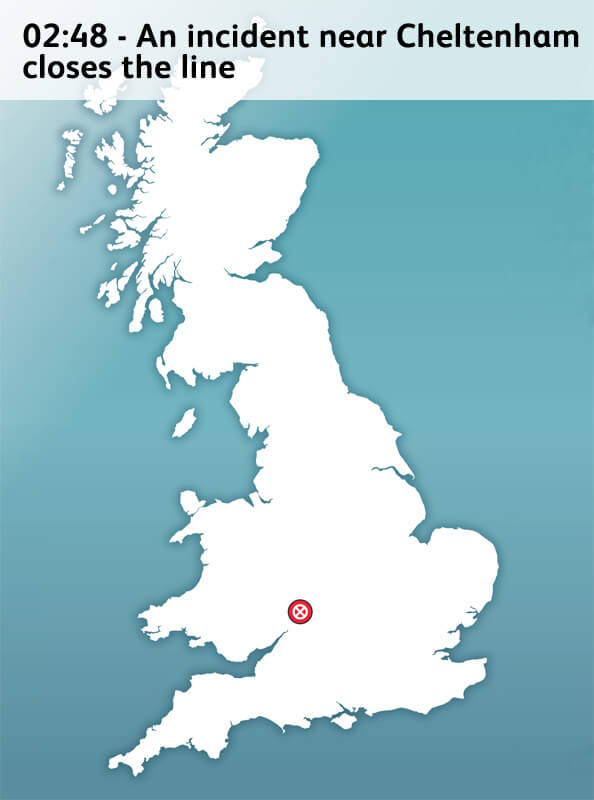
\includegraphics[width=3.5cm]{images/Knock-on-delays-1.jpg} }}
    \quad
    \subfloat[08:48]{{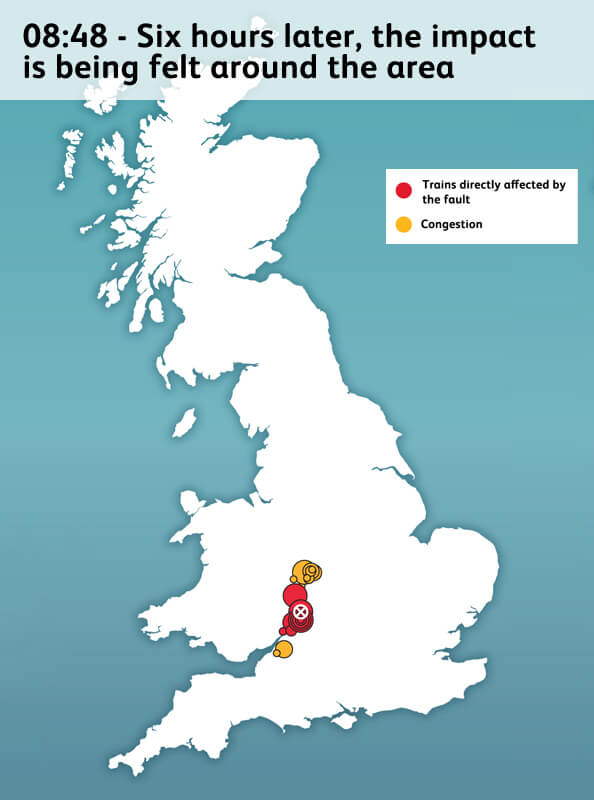
\includegraphics[width=3.5cm]{images/Knock-on-delays-2.jpg} }}
    \quad
    \subfloat[15:18]{{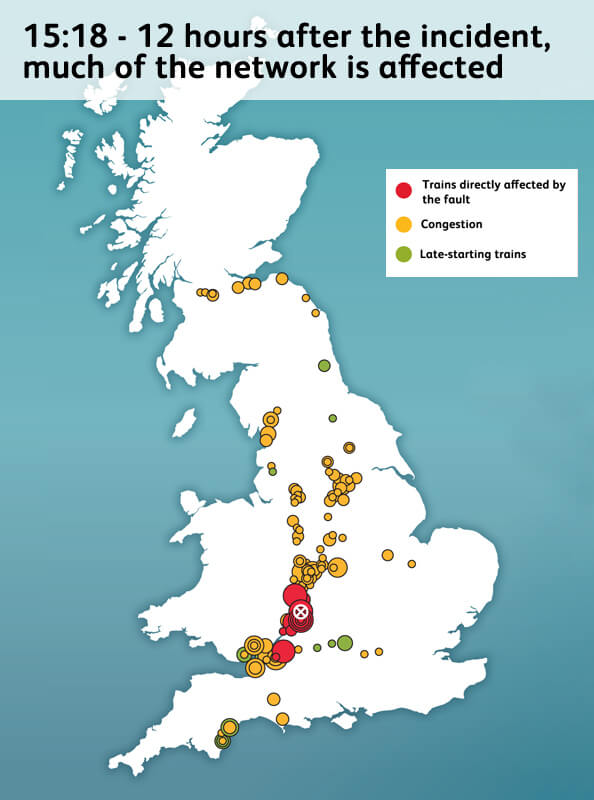
\includegraphics[width=3.5cm]{images/Knock-on-delays-3.jpg} }}
    \quad
    \subfloat[22:48]{{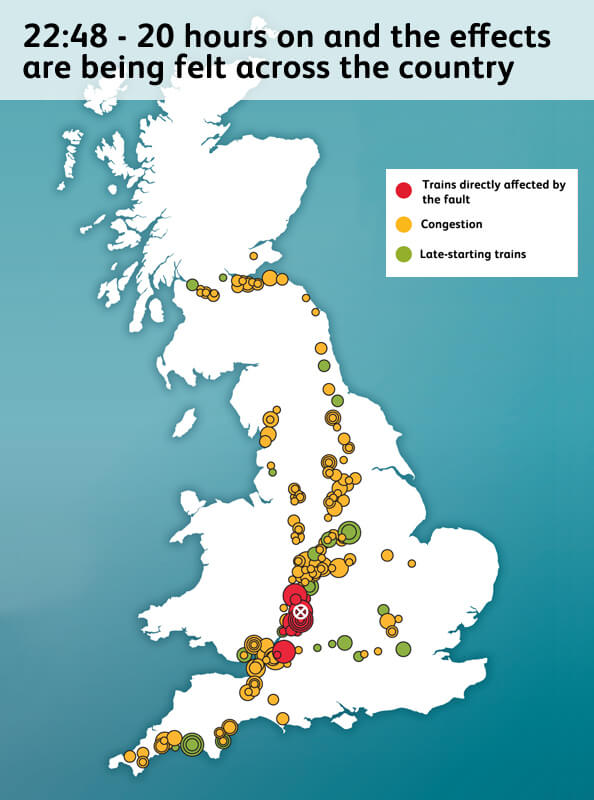
\includegraphics[width=3.5cm]{images/Knock-on-delays-4.jpg} }}
    \caption{A visualisation of delay propagation. A single incident at 02:48 causes congestions, delays and cancellations across most of the country for the next $24$ hours. Red dots are trains directly affected by the fault; yellow, congestion; and green, late-running trains.}
    \label{fig:delay_propagation}
\end{figure}

Data is exogenous if it is independent of other input data but the output is dependent upon it. In the context of primary delay prediction, the more of the causes of primary delay that can be incorporated into a model, the better it will perform. Models tend to use a combination of infrastructure \cite{markovic_et_al_2015,milinkovic_et_al_2013,lessan_fu_wen_2019}, weather \cite{oneto_et_al_2016,wang_zhang_2019,oneto_et_al_2017,lessan_fu_wen_2019}, expert opinions \cite{markovic_et_al_2015,oneto_et_al_2019} and engineering work \cite{lessan_fu_wen_2019}. Information about passenger flows and railway asset conditions is also useful \cite{oneto_et_al_2017}. Where directly relevant exogenous data is unavailable, it is possible to use proxies (Harris, 1992), such as: 

\begin{itemize}
	\item{train length (as a proxy for the number of doors to manage, and passenger demand)}
	\item{distance covered (as a proxy for the likelihood of encountering track defects and other technical / operational problems)}
	\item{the previous number of stops (as a proxy for cumulative delay resulting from passengers alighting and boarding)}
	\item{the age of the motive power unit (as a proxy for reliability)}
	\item{track occupation (as a proxy for capacity utilisation of the railway, and thus the likelihood of delays propagating)}
\end{itemize}

\subsection{Objectives}

The research question proposed is: \textit{can medium-term train delays be predicted}? To address this question, the objectives for this project were divided into three categories: minimum, intermediate, and advanced. 

The minimum objective of this project is to construct a high-quality dataset incorporating a variety of exogenous data. The purpose of this objective is twofold. Such a dataset is, first and foremost, a prerequisite for machine learning, and there are none publicly available. There are few objective criteria for what makes a good dataset, save that it ought to be clean, logically structured, and complete, with only relevant fields included.

The intermediate objective is to develop a binary classification model to predict whether a train will be delayed. A variety of classification models will be selected, with selection informed by a literature review.

The advanced objective is to build upon the intermediate objective by extensively testing and fine-tuning the best-performing model using cross validation and hyperparameter optimisation.

\section{Related Work}
\label{section:related_work}

In the section, we present work related to our research question: \textit{Can medium-term train delays be predicted?}. Although there has been significant academic effort into producing real-time train delay prediction (TDP) systems, research on medium-term TDP is rather sparse. Fortunately, there is considerable overlap between the two timeframes. Solutions to the problem of real-time TDP use a variety of machine learning regression models, with the field tending towards ensembles / hybrids  and random forests. The inclusion of exogenous data pertaining to weather and infrastructure is also popular.  There are many classifications of TDP models, based on scope, model type, and solution methods \cite{markovic_et_al_2015}. Generally, approaches may be divided using two axes: whether they are offline or online, and whether they use analytical or data-driven models. As this project is concerned with latter, the former is discussed only briefly. Online models are updated with new data as it becomes available; data-driven models are trained using historical data.

\subsection{Analytical approaches}

An analytical model is “primarily quantitative or computational in nature and represents the system in terms of a set of mathematical equations that specify parametric relationships and their associated parameter values as a function of time, space, and/or other system parameters” \cite{friedenthal_moore_steiner_2012}. Current state-of-the-art train delay prediction systems use analytical models \cite{oneto_et_al_2016}: “static rules, built by experts on railway infrastructure, and based on classical univariate statistics”.

Simplistic early models, such as those developed by \cite{frank_1966} make overly restrictive assumptions about railway operations, e.g. no overtakes are allowed, departure times are uniformly distributed, and that the speed of each train is unique and constant. Subsequent work in this area has largely relaxed these assumptions by including factors such as overtakes, different speeds, priority systems, and uncertainties associated with train departure time \cite{petersen_1974,chen_harker_1990}. Further models have become increasingly advanced, incorporating stochastic approximation \cite{carey_kwiecinski_1994}, and the impacts of dispatching strategies on train delays and passenger waiting time.

Much work has also been done which blurs the line between analyitical and data-driven models \cite{kecman_corman_meng_2015,corman_kecman_2018} by using stochastic models based on Bayesian networks and trained on historical data to predict delays, with considerable success. However, there is a fundamental limit on the complexity of analytical models, and as the field of machine learning has matured, the applicability of data-driven models to TDP has been increasingly well explored. 

\subsection{Online / dynamic data-driven approaches}

Most real-time TDP systems are online. The first comprehensive attempt at developing a TDP system was made by Oneto et al. (2016). Subsequent papers \cite{oneto_et_al_2017,oneto_et_al_2019} have expanded the proposed models in scope and performance.
The authors consider a rail network a graph, where nodes represent checkpoints and edges tracks connecting them. A train follows an itinerary composed of $N_c$ checkpoints characterised by an origin, a terminus, and intermediate locations such as stops and transits. A schedule is modelled as a time series forecast problem, with performance at previous checkpoints used to predict performance at subsequent checkpoints. A model for each train is trained using historical delay data. The authors tested random forests (RF), Extreme Learning Machines (ELM), and Kernel Methods (KM) and found that their RF performed twice as well as current state-of-the-art TDP systems. The inclusion of weather further improved accuracy by approximately 10\%. Their model was very computationally expensive, however, requiring approximately 600,000 models to be trained daily across the entire rail network. 

The authors then generalise their work to produce a dynamic data-driven TDP system \cite{oneto_et_al_2017}, with performance tuned using Thresholdout, which reduces overfitting. They compare the performance of two implementations of shallow and deep ELMs. 
This work laid the groundwork for their most recent paper \cite{oneto_et_al_2019}, which combines an experience-based model (EBM) and multiple RFs into a hybrid model (HM). The EBM uses operators’ knowledge and experience of the network to inform features. As Martin (2016) notes, in real-world train operations, delay prediction relies heavily on the experience and intuition of a local dispatcher, rather than a network-wide computational instrument. The HM is a decision tree where each leaf is a RF. Trains are directed to the appropriate RF by similarity, eliminating the need for a model for every train. A new leaf is added each time a new train is seen that belongs to a previously unexplored branch of the decision tree. The RF regressor in the leaf is trained based on all the past train movements in that leaf. Trains older than 3 months are ‘forgotten’, to keep the size of the model constrained. Furthermore, this model naturally handles the mercurial nature of train schedules, which are both released periodically and revised constantly. The model requires only 10 days’ of data after a new schedule comes into effect to reach optimal accuracy, with excellent performance also noted for outliers. The HM offers the best trade-off between accuracy and computational requirements, with superior results to all current models. 

A similarly impressive model was developed by Lessan \textit{et al.} \cite{lessan_fu_wen_2019}, working closely with Deutsche Bahn (DB). The authors used $3.25$ years’ of data from DB and incorporated a wide range of exogenous data, with approximately $350$ features for operational (i.e. currently running) trains and $70$ for non-operational trains. The authors tested support vector regression (SVR) but settled on RFs. Three models were used for operational trains: an online RF, mesoscopic simulation, and kernel regression. Two were used for non-operational trains: an offline RF and mesoscopic simulation. The authors found an accuracy of over $80\%$ in predictions within a $60$-minute horizon, a considerable improvement in real-time forecasts, but found that beyond that horizon predictions were only marginally better than the schedule.

\subsection{Offline / static data-driven approaches}

Static models are not updated with data as it comes available. Early attempts used simple neural networks \cite{peters_et_al_2005} and were essentially proofs-of-concept. The use of neural networks was further investigated by Yaghini \textit{et al.} \cite{yaghini_et_al_2013} using data from Iranian Railways to predict the late arrival of passenger trains. Their model performed better to alternatives such as decision trees and logistic regression. The authors also tested the impact of various encoding schemes. 

Subsequent work is largely exploratory, with no clear sense of progression as described in the previous section. Papers investigate a wide variety of models, such as Fuzzy Petri Nets (FPNs) \cite{milinkovic_et_al_2013}, support vector regression (SVM) \cite{markovic_et_al_2015} logistic regression \cite{wang_work_2015} and gradient-boosted random forests \cite{wang__and_zhang_2015}.

Milinkovic \textit{et al.} \cite{milinkovic_et_al_2013} presented the first use of an FPN. The authors explored two separate FPNs. In the first, expert knowledge was used to define fuzzy sets and rules. In the second, an Adaptive Network Fuzzy Inference System (ANFIS) was trained on historical delay data and then replicated in an FPN. Both were then tested with real data from a Belgrade station node. The ANFIS-FPN produced results within 5\% of actual delay values for a subset of the data; slightly worse performance was observed for the expert-defined FPN.

Markovic \textit{et al.} \cite{markovic_et_al_2015} presented the first use of SVM. They found it outperformed artificial neural networks. Data for the analysis was again collected from Serbian Railways. The paper used the expert opinions of dispatchers to estimate the likelihood of multiple factors along a rail line, such as single-tracking, junctions, or the number of stations, causing a delay, using the Delphi method to obtain a final estimate. A strong correlation was found between expert opinions and train delays. The focus was on developing a functional relationship between delays and infrastructure so the effect of infrastructure improvements on delays can be predicted and valued.  

Wang and Work \cite{wang_work_2015} used data from Amtrak to develop two vector autoregression models: one offline, the other online. The offline model improved the RMSE of predicted delays by $12\%$; the online model, by $60\%$.

Wang and Zhang \cite{wang_zhang_2019} present a relatively simple gradient-boosted regression trees (GBRT) model. The model was trained on a three-month dataset of weather, train delay, and train schedule records. Their model can make predictions up to 10 days’ in advance, the limit of the weather forecast system used, but performed poorly, which the authors attribute to the limited size of their dataset. This paper most closely resembles the objectives of this project. 

\section{Solution}
\label{section:solution}

In this solution we present our solution to constructing a dataset and identifying a suitable binary classification model. The \verb|Python| programming language was used throughout, with \verb|NumPy| for numerical operations, \verb|Pandas| for data manipulation and analysis, \verb|scikit-learn| for machine learning, and \verb|Matplotlib| for graphing. 

\subsection{Dataset construction: the Extract-Transform-Load (ETL) pipeline}

Central to the importance of machine learning is a high-quality labelled dataset. Unfortunately, there are no publicly available datasets for train delay. Correspondence between authors of previous papers \cite{yaghini_et_al_2013,wang_zhang_2019} proved unfruitful, so it was necessary to construct a new dataset, which became the minimum objective of this project. Dataset construction is a complex task. It falls under the purview of the Extract-Transform-Load (ETL) pipeline\footnote{Sometimes a different order is used: Extract-Load-Transform (ELT). The sole difference is where the transformation stage takes place. The distinction is largely academic here, so ETL is used throughout.}. This pipeline extracts data from sources, transforms them into a usable format, and loads them into storage for future operations. It is a very time-consuming task; “it is not uncommon for a project team to spend as much as $50\%$ to $70\%$ of project effort on ETL functions” \cite[p.~284]{ponniah_2010}. This proved the case with this project, so we dedicate considerable space to explaining each stage in the pipeline, and how it was realised in the context of this dissertation.

First, we identified suitable data sources for the train data itself (schedules, location, and movement) and the three classes of primary delay (weather, infrastructure, and engineering) identified in Section~\ref{section:introduction} (\ref{subsection:background}). The UK rail infrastructure manager Network Rail (NR) opened its feeds\footnote{https://www.networkrail.co.uk/who-we-are/transparency-and-ethics/transparency/open-data-feeds/} to developer usage in $2011$; they are presented in Table~\ref{table:nr_feeds}.

\begin{table}[htb]
\centering
\caption{NR data feeds and their use in this project. I = investigated, U = used, N = not used.}
\label{table:nr_feeds}
\begin{tabular}{|l|p{9cm}|p{2cm}|c|}
\hline
\textbf{Acronym} & \textbf{Description} & \textbf{Frequency} & \multicolumn{1}{l|}{\textbf{Usage}} \\ \hline
BPLAN & Train planning data, including locations and sectional running times. & Twice a year & I \\ \hline
CORPUS & Location reference data. & Monthly & U \\ \hline
MOVEMENT & Train positioning and movement event data. & Real-time & U \\ \hline
RTPPM & Performance of trains against the timetable, measured as the percentage of trains arriving at their destination on-time. & Once a minute         & N \\ \hline
SCHEDULE         & Daily extracts and updates of train schedules from the Integrated Train Planning System (ITPS).                          & Overnight each night  & U                                       \\ \hline
SMART            & Train describer berth offset data used for train reporting.                                                              & Monthly               & N                                       \\ \hline
TD               & Train positioning data at a signalling berth level.                                                                      & Real-time             & N                                       \\ \hline
TSR              & Details of temporary reductions in permissible speed across the rail network.                                            & Weekly (on Friday) & I                                       \\ \hline
VSTP             & Train schedules created via the VSTP process                                                                             & Real-time             & I                                       \\ \hline
\end{tabular}
\end{table}

\subsubsection{Schedules: SCHEDULE}

Schedules are available as CIFs\footnote{Common Interface File} from the SCHEDULE feed. A full CIF – a database snapshot – is released every Friday morning, with update CIFs released every morning. Each update must be applied to the latest full CIF to maintain a correct database. Each file contains train schedules, metadata, and associations. We ideally would have used the VSTP feed as well, which refers to trains scheduled up to $48$ hours before they are due to run. However, the feed was not archived in the repository from which we sourced the rest of our data.

\subsubsection{Location: CORPUS (and NaPTAN)}

CORPUS is used in conjunction with the National Public Transport Access Node (NaPTAN) database, a nationwide system for uniquely identifying all points of access (nodes) to public transport in the UK. Only rail stations are, naturally, of concern here. A large variety of codes are used to refer to locations in the UK rail network; they are presented in Table~\ref{table:codes}.

\subsubsection{Movement: TD, TRUST, and Darwin}

The TD feed provides information about the position of trains through a network of berths. A berth usually represents a signal. We discarded TD as too low-level for this project. There are two movement systems currently in by NR: Train Running Under System TOPS (TRUST) and Darwin. TRUST is a NR system used for monitoring the progress of trains and tracking delays in the UK. Darwin uses both TRUST and TD for real-time data, and also incorporates Darwin workstations, Customer Information Systems (CIS), and internal messaging systems.

TD feeds into TRUST, and TRUST into DARWIN. Darwin provides more comprehensive information. While the objectives of this project were being defined, it was undecided whether to focus on real-time or medium-term train delays. The real-time timeframe would have necessitated the use of Darwin, whereas medium-term could have used either. To keep options open, Darwin was therefore used. Darwin messages contain a lot of extraneous information, but fundamentally each movement message contains a timestamp and a location, either a STANOX or TIPLOC. Both CORPUS and NaPTAN are therefore necessary to ensure a message can be geolocated.

\begin{table}[h!]
\centering
\caption{UK rail network location codes.}
\label{table:codes}
\begin{tabular}{|p{2.5cm}|c|c|p{8.5cm}|}
\hline
\textbf{}          & \multicolumn{1}{l|}{\textbf{CORPUS}} & \multicolumn{1}{l|}{\textbf{NaPTAN}} & \textbf{Description}                                                                                                                                                                \\ \hline
STANOX             & Y                                    &                                      & Station Number. First two digits are the geographic area. Can refer to non-station locations such as sidings and junctions. Numbers run broadly north-to-south.                     \\ \hline
UIC                & Y                                    &                                      &                                                                                                                                                                                     \\ \hline
CRS / NRS / 3ALPHA & Y                                    & Y                                    & Used primarily to identify stations and on seat reservation labels.                                                                                                                 \\ \hline
TIPLOC             & Y                                    & Y                                    & Timing Point Location. Relates to points used in deriving train schedules. A station often has multiple TIPLOCs if it consists of  multiple groups of platforms on different lines. \\ \hline
NLC                & Y                                    &                                      & National  Location Code. Identifies locations on the railway. Used for retailing and accounting purposes.                                                                           \\ \hline
NLCDESC            & Y                                    &                                      & A description of the NLC.                                                                                                                                                           \\ \hline
NLCDESC16          & Y                                    &                                      & A description of the NLC.                                                                                                                                                           \\ \hline
ATCO               &                                      & Y                                    &                                                                                                                                                                                     \\ \hline
EASTING, NORTHING  &                                      & Y                                    & Geographic Cartesian coordinates for a point. Uses EPSG:27700\footnote{https://epsg.io/27700}, the British National Grid / Ordnance Survey system.                                                                  \\ \hline
NAME               &                                      & Y                                    & The name of the location.                                                                                                                                                           \\ \hline
\end{tabular}
\end{table}

\subsubsection{Weather: MIDAS, CEDA, and Datapoint}

The primary source of weather data is the Met Office Integrated Data Archive System (MIDAS). MIDAS is a database of land and marine surface observations, collected from 1853 to the present day, by the Met Office station network. MIDAS offers several datasets. The most comprehensive is the Hourly Weather Observation Data, which contains meteorological values measured on an hourly time scale. These observations include 104 fields , though many are for quality control, or too specific to necessitate inclusion. Station data is available from the Centre for Environmental Data Analysis (CEDA). Each station is geolocated by latitude and longitude. For this project to be of practical use, trained models must be applicable to unseen data. Unseen train data are simply train schedules; unseen weather data are forecasts. Forecasts are available from Met Office Datapoint, a service allowing access to freely available Met Office data feeds. They may be obtained as 3-hourly site-specific forecasts up to 5 days’ in advance. There are 10 forecast available fields. 

\subsubsection{Infrastructure: BPLAN and the Train Planning Network Model}

The Train Planning Network Model is used by the Integrated Train Planning System (ITPS). We were unable to integrate either of these datasets, as there was too little pubicly available documentation.

\subsubsection{Engineering: TSR}

TSR provides proxy details of engineering works. It was not archived in the repository from which we sourced the rest of our NR data, so we could not make sure of it.

\subsection{Extraction}

Extraction is the process of collecting data, often from multiple different sources, and moving it to a \textit{staging area}. Some basic validation also takes place at this stage. The extraction process of the each data source is presented in Table~\ref{table:extraction}.

\begin{table}[htb]
\centering
\caption{Extraction methods for each data source}
\label{table:extraction}
\begin{tabular}{|l|p{12cm}|}
\hline
\textbf{Data source} & \textbf{Notes}                                                                                                                                                                                                                                                                                                                                                                                                                                                                                                                                                                                                                                           \\ \hline
Schedule            & Schedule data is available from Peter Hicks’ website . Both full and update extracts are downloaded as gzipped files.                                                                                                                                                                                                                                                                                                                                                                                                                                                                                                                                    \\ \hline
Movement            & Darwin data is also available from Peter Hicks’ website . Each day is a bzip2-compressed tar file containing 1440 files, one for each minute in the day. Each file comprises XML messages. Each minute is extracted in memory and written to one CSV for each day / file.                                                                                                                                                                                                                                                                                                                                                                                \\ \hline
Location            & NaPTAN is available as a zipped CSV from the Department for Transport (DfT). Only the railway nodes are extracted and saved. CORPUS is available from NR as a gzipped JSON. Only the TIPLOC information is extracted and saved.                                                                                                                                                                                                                                                                                                                                                                                                                          \\ \hline
Weather             & Available for download as a CSV file, via FTP from CEDA, though headers must be downloaded separately. Station data is also available from CEDA as a KMZ file\footnote{A KMZ file is a zipped KML (Keyhole Markup Language) file; KML is an XML notation for expressing geographic annotations and visualisations.}. The KMZ file is parsed using pykml and station metadata using BeautifulSoup to produce a CSV. \\ \hline
\end{tabular}
\end{table}

\subsection{Transform}

Transformation is the process of applying a set of functions to extracted data, to clean, map, validate, and consolidate datasets, with the aim of making the data conform to a uniform schema. There is a lot of overlap between transformation and preprocessing, the stage just prior to training. The difference lies in ease of repetition: transformation would, ideally, be performed once, as operations are typically expensive, operating on vast quantities of unstructured and semi-structured data, where preprocessing, using heavily optimised code in NumPy and Pandas, can be iteratively developed.

\subsubsection{Transforming schedules}

Train scheduling is a very complex problem. As we mentioned, an update CIF is released every morning. It contains deletions, amendments, and new schedules, which must be applied to the currently-held schedule database. After each update is applied, the schedules for that day are written to file. Full schedules are released weekly, so errors cannot propagate for more than $7$ days. A CIF contains $9$ types of record. We used $5$ of these records to build, for each train, a single row containing metadata, such as the TOC responsible for the train, location data, such as the origin, destination, and number of stops, and datetime data, such as the scheduled departure (from the origin) datetime and the scheduled arrival (at the terminus) datetime. 

We discarded $2$ types of record to reduce complexity: CRs (change en route) and AAs (associations). An association represents some dependency between two trains, such as crew or engines. They have the potential to be a rich source of data - is, for instance, a train with more associations more likely to be delayed? - but including them would necessitate a much more complex model than the simpler tabular format suitable for machine learning. A change en route indicates that some metadata has changed during a train's journey. Some changes are typically small - a change in seating rules, for instance, or whether reservations are required - and including them would again necessitate a more complex model and greater space requirements. As we believed the impact of CRs would be small, we ignored them.

\subsubsection{Transforming weather}

As mentioned previously, there is a need to map from the MIDAS format to DataPoint format. There are $10$ available DataPoint fields for forecasts, of which only $7$ could be meaningfully mapped to equivalent MIDAS fields. For several, this was a simple unit conversion. For visibility and weather type, predefined codes were used to establish a map between the two formats\footnote{https://www.metoffice.gov.uk/services/data/datapoint/code-definitions}. 

\subsubsection{Transforming movement}

Each day of train movements is a file roughly \verb|1.5GB| in size. This file also contains a variety of other messages: forecasts, schedules, station messages, alarms, warnings, and so on. We converted each train movement into a simple record comprising the type, train, location, and time the movement took place. DARWIN does not include the date at which the movement took place, so this was inferred from other metadata. We also dropped duplicate messages.

\subsubsection{Transforming location}

This stage was relatively simple. We merged NaPTAN and CORPUS, and calculated the closest geographical weather stations in MIDAS for future use.. 

\subsection{Load}

Load is the process of storing data in a format accessible for future usage. It was a more complex in this project, involving the merging of the aforementioned datasets. We joined together schedule and movement data and constructed a target column, \verb|delayed|, using the the difference between the scheduled arrival time and actual arrival time. We discarded erroneous rows and dropped irrelevant columns. We then joined location data and weather data. 

\subsection{Model selection}
\label{subsection:model_selection}

When searching for candidate models, we looked mainly at those with generally good performance at classification tasks, rather than those identified in Section~\ref{section:related_work}, though there was some overlap \cite{wang_zhang_2019,wang_work_2015}. This is because, as discussed earlier, the majority of research into TDP focuses on the real-time timeframe, not the medium-term, and so are not applicable. As this process is exploratory, we chose a wide range of models. As ensembles have proven popular, we focused on those. We also selected several simple linear models, anticipating poor performance, for comparison. For ease of testing, we only used models available in \verb|scikit-learn|. $10$ models were chosen for the initial round: an AdaBoost classifier, a decision tree classifier, a Gaussian NB classifier, a gradient-boosting classifier, a histogram-gradient-boosting classifier, a linear Support Vector Classifier (SVC), logistic regression, a random forest classifier, a ridge classifier, and a stochastic gradient descent (SGD) classifier.

\clearpage
\section{Results}

In this section, we present the results of our ETL pipeline, our classification model, and our hyperparameter optimisation. We also discuss the metrics used to analyse results. We trained and tested each of the models identified in Section~\ref{section:solution} (\ref{subsection:model_selection}) on the dataset produced by our ETL pipeline, after some transformations and resampling. We further analysed the best-performing model to identify important features, and subjected it to an hyperparameter optimisation process to improve performance. The experiment environment system specification is outlined in Table~\ref{table:experiment}.

\begin{table}[htb]
\centering
\caption{Experiment environment system specification}
\label{table:experiment}
\begin{tabular}{|l|l|}
\hline
{\bf Component} & {\bf Details}                     \\ \hline
Processor & Intel Core i5-6990K 3.6 GHz \\ \hline
GPU       & NVIDIA GeForce 980 TI 8GB   \\ \hline
RAM       & 32 GB 2400 MHz DIMM         \\ \hline
OS        & Windows 10                  \\ \hline
\end{tabular}
\end{table}

\subsection{ETL}

The output of our ETL pipeline is a single CSV, \verb|1.1 GB| in size, containing approximately $5.2$ million rows and $47$ columns, over a period of one year (\verb|2018-04-01| to \verb|2019-04-031|). Approximately $20,000$ trains run a day in the UK, and we were successful in capturing approximately $76\%$. The numeric, categorical, and datetime fields prior to transformation and resampling are presented in Tables~\ref{table:etl_numeric},~\ref{table:etl_categorical}, and~\ref{table:etl_datetime}, respectively. We can observe, for instance, that the busiest TIPLOC is \verb|LIVST| (Liverpool Street); that the mean speed of trains in the UK is $89.5$ mph; and that the single busiest time (for departures) was \verb|2019-03-15 07:30:00|.

Before testing our models, we preprocessed our dataset. We encoded datetime data cyclically, whereby each datetime is split into its constituent parts and each part is converted into two values, one for \verb|sin| and one for \verb|cos|, such that each is encoded as a point on unit circle. For compatibility between different models, we one-hot encoded categorical variables and scaled numeric variables to Gaussian; we later relax this requirement. We also resampled the dataset. Approximately $10\%$ of rows are positive (i.e. delayed). This causes poor performance: a model can learn to always predict negative (i.e. not delayed) to trivially achieve approximately $90$\% accuracy. To remedy this we investigated different ways to balance the dataset, and chose to oversample the minority class (i.e. delayed) using SMOTE \cite{chawla_et_al_2002} and randomly undersample the majority class (i.e. not delayed) to achieve a 50:50 ratio. The final form of our dataset is a $(1178694, 283)$ sparse matrix. 

\begin{table}[]
\centering
\caption{Numeric fields in the dataset}
\label{table:etl_numeric}
\begin{tabular}{|l|l|r|r|r|r|r|}
\hline
                       & dtype  & \multicolumn{1}{l|}{no. col} & \multicolumn{1}{l|}{mean} & \multicolumn{1}{l|}{std} & \multicolumn{1}{l|}{min} & \multicolumn{1}{l|}{max} \\ \hline
speed                  & int    &                                  & 8.951162e+01              & 1.442622e+01             & 45                       & 140                      \\ \hline
length                 & int    &                                  & 1.830134e+01              & 1.266664e+01             & 2                        & 150                      \\ \hline
duration               & float  &                                  & 6.482278e+01              & 5.540015e+01             & 1                        & 803                      \\ \hline
delay                  & float  &                                  & 1.464341e+01              & 1.420186e+02             & -412.5                   & 2492.5                   \\ \hline
freight                & binary &                                  & 1.016241e-04              & 1.008037e-02             & 0                        & 1                        \\ \hline
delayed                & binary &                                  & 1.132171e-01              & 3.168581e-01             & 0                        & 1                        \\ \hline
bank\_holiday\_running & binary &                                  & 9.999364e-01              & 7.973899e-03             & 0                        & 1                        \\ \hline
mon - sun              & binary & 7                                &                           &                          &                          &                          \\ \hline
characteristic         & binary & 12                               &                           &                          &                          &                          \\ \hline
catering               & binary & 6                                &                           &                          &                          &                          \\ \hline
\end{tabular}
\end{table}

\begin{table}[]
\centering
\caption{Categorical fields in the dataset}
\label{table:etl_categorical}
\begin{tabular}{|l|r|r|r|}
\hline
                          & \multicolumn{1}{l|}{unique} & \multicolumn{1}{l|}{top} & \multicolumn{1}{l|}{freq} \\ \hline
status                    & 2                           & P                        & 5156231                   \\ \hline
category                  & 10                          & OO                       & 3530949                   \\ \hline
power\_type               & 5                           & EMU                      & 2786544                   \\ \hline
timing\_load              & 38                          & S                        & 898631                    \\ \hline
seating                   & 2                           & S                        & 3565386                   \\ \hline
reservations              & 3                           & S                        & 984770                    \\ \hline
origin                    & 683                         & LIVST                    & 180355                    \\ \hline
destination               & 654                         & LIVST                    & 181829                    \\ \hline
ATOC\_code                & 33                          & NT                       & 784180                    \\ \hline
origin\_stanox\_area      & 80                          & 88                       & 372775                    \\ \hline
destination\_stanox\_area & 80                          & 88                       & 372528                    \\ \hline
\end{tabular}
\end{table}

\begin{table}[]
\centering
\caption{Datetime fields in the dataset}
\label{table:etl_datetime}
\begin{tabular}{|l|r|r|r|r|r|}
\hline
    & \multicolumn{1}{l|}{unique} & \multicolumn{1}{l|}{top} & \multicolumn{1}{l|}{freq} & \multicolumn{1}{l|}{first} & \multicolumn{1}{l|}{last} \\ \hline
std & 432969                      & 2018-04-30 07:00:30      & 52                        & 2018-04-01 00:08:30        & 2019-03-31 23:59:30       \\ \hline
sta & 436717                      & 2019-03-18 16:44:30      & 34                        & 2018-04-01 00:12:30        & 2019-04-01 09:03:30       \\ \hline
atd & 436262                      & 2019-03-15 07:30:00      & 45                        & 2018-04-01 00:06:00        & 2019-04-01 11:42:00       \\ \hline
ata & 437485                      & 2019-03-30 10:36:00      & 38                        & 2018-04-01 00:11:00        & 2019-04-01 12:00:00       \\ \hline
\end{tabular}
\end{table}


\subsection{Binary classification}

To evaluate our models, we will produce accuracy (Acc), precision (Prec), and recall (Rec) statistics using the number of true positive (TP), true negative (TN), false positive (FP), and false negative (FN) classifications of our models. We also use the $F_\beta$-measure (Eq.~\ref{equation:f_measure}). The $F_\beta$-measure is the weighted harmonic mean of precision and recall, which captures the natural trade-off between them. A $\beta$ of $1$ indicates that Prec and Rec are weighted equally importantly.

\begin{equation}
\label{equation:f_measure}
F_\beta = (1 + \beta) \frac{precision \cdot recall}{\beta^2 \cdot (precision + recall)}
\end{equation}

 We trained each of the models identified in Section~\ref{section:solution} (\ref{subsection:model_selection}) on the same $70\%$ of the dataset. No limits were imposed on memory, CPU usage, or time. Two potential models were discarded for incompatibility with the sparse matrix: GaussianNB and HistGradientBoostingClassifier. We then tested the remaining models on the remaining $30\%$ of the dataset, and computed a number of metrics. The results are displayed in Table~\ref{table:results_explore}.

\begin{table}[htb]
\centering
\caption{A full statistical analysis of each model after training on the test dataset}
\label{table:results_explore}
\begin{tabular}{|p{5cm}|c|c|c|c|}
\hline
\textbf{Model}                  & \multicolumn{1}{l|}{\textbf{Acc}} & \multicolumn{1}{l|}{\textbf{Prec}} & \multicolumn{1}{l|}{\textbf{Rec}} & \multicolumn{1}{l|}{\textbf{$F_1$}} \\ \hline
AdaBoostClassifier              & 0.67                              & 0.62                               & 0.67                              & 0.67                               \\ \hline
DecisionTreeClassifier          & 0.68                              & 0.62                               & 0.69                              & 0.68                               \\ \hline
GradientBoostingClassifier      & 0.68                              & 0.63                               & 0.67                              & 0.68                               \\ \hline
LinearSVC                       & 0.67                              & 0.61                               & 0.67                              & 0.67                               \\ \hline
LogisticRegression              & 0.67                              & 0.61                               & 0.67                              & 0.67                               \\ \hline
MLPClassifier                   &\textbf{0.73}                              & 0.67                               & 0.73                              & 0.73                               \\ \hline
\textbf{RandomForestClassifier} & \textbf{0.73}                     & \textbf{0.70}                      & \textbf{0.74}                     & \textbf{0.74}                      \\ \hline
RidgeClassifier                 & 0.67                              & 0.61                               & 0.67                              & 0.67                               \\ \hline
SGDClassifier                   & 0.66                              & 0.60                               & 0.66                              & 0.66                               \\ \hline
\end{tabular}
\end{table}

Table~\ref{table:results_explore} shows that the random forest is the superior model for solving this binary classification problem, with the greatest recall, precision, accuracy and $F_1$-measure. The MLPClassifier (a multi-layer Perceptron classifier, a type of neural network) also performed well. Interestingly, the simple models achieved comparable performance to the random forest in a fraction of the training time - under $10$ seconds, in the case of the LinearSVC.  Based on these results, we investigated random forests further.

\subsection{Random forests}

Random forests (RFs) are ensembles consisting of multiple random decision trees. Each tree is built on a random subset of the original data; at each tree node, a random subset of features are randomly selected to generate the best fit. They do not require feature scaling or categorical feature encoding, so we simplified the pipeline by removing these features. We then identified five hyperparameters likely to impact performance and used randomised search combined with $3$-fold cross validation to optimise them; the results are presented in Table~\ref{table:results_parameters}.

\begin{table}[h!]
\centering
\caption{Random forest hyperparameter optimisation}
\label{table:results_parameters}
\begin{tabular}{|l|p{7cm}|c|c|}
\hline
\textbf{Hyperparameter} & \textbf{Function}                                                  & \multicolumn{1}{l|}{\textbf{Default}} & \multicolumn{1}{l|}{\textbf{Optimum}} \\ \hline
\verb|n_estimators|           & Number of trees in the forest                                      & 100                                   & 200                                   \\ \hline
\verb|max_features|           & The number of features to consider when looking for the best split & auto                                  & sqrt                                  \\ \hline
\verb|max_depth|              & The maximum depth of the tree                                      & None                                  & 10                                    \\ \hline
\verb|min_samples_split|     & The number of samples required to split an internal node           & 2                                     & 10                                    \\ \hline
\verb|min_samples_leaf|      & The minimum number of samples required to be a leaf node           & 1                                     & 2                                     \\ \hline
\verb|bootstrap|               & Whether bootstrap samples are used when building trees             & True                                  & False                                 \\ \hline
\end{tabular}
\end{table}

We achieved a modest improvement in performance through this process, with all metrics showing an improvement of between $2.70\%$ and $8.57\%$ (in the case of precision), as presented in Table~\ref{table:results_tune}. Random forests are typically difficult to fine-tune, so this small improvement was expected.

\begin{table}[htb]
\centering
\caption{A statistical analysis of the tuned random forest}
\label{table:results_tune}
\begin{tabular}{|p{5cm}|c|c|c|c|}
\hline
\textbf{Model}                  & \multicolumn{1}{l|}{\textbf{Acc}} & \multicolumn{1}{l|}{\textbf{Prec}} & \multicolumn{1}{l|}{\textbf{Rec}} & \multicolumn{1}{l|}{\textbf{$F_1$}} \\ \hline
RandomForestClassifier & 0.76                     & 0.76                      & 0.76                     & 0.76                      \\ \hline
\end{tabular}
\end{table}

Finally, we evaluated the model using repeated stratified $10$-fold cross validation, which selects folds so that each contains roughly the same class distribution in the original dataset (in this case, the re-sampled dataset). The results are plotted in Figure~\ref{fig:roc} as a $ROC_{AUC}$ curve. $ROC$ curves visualise the trade-off between the true positive rate (TPR) and false positive rate (FPR) for a predictive model using different probability thresholds. A larger area under the curve ($AUC$) is better. We obtained a mean $ROC_{AUC}$ of $0.77 \pm 0.00$. This is because our dataset was perfectly balanced, and sufficiently large that there was essentially no difference between the folds.  

\begin{figure}[h!]
  \centering
  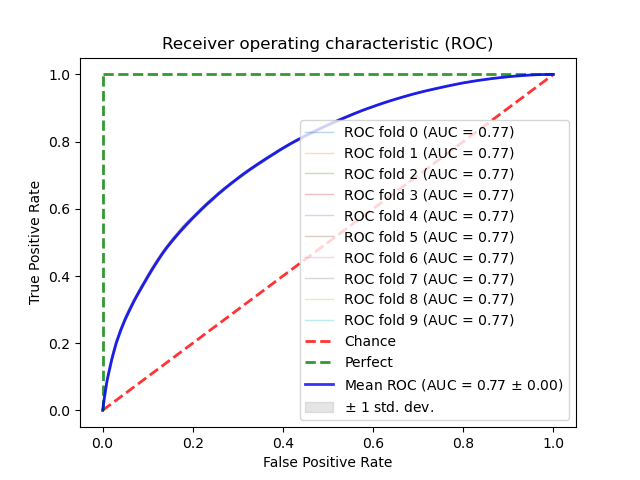
\includegraphics[width=0.85\linewidth,height=0.5\textheight,keepaspectratio]{images/roc_auc_10.png}
  \caption{A ROC\textsubscript{AUC} graph.}
  \label{fig:roc}
\end{figure}

\subsection{Exogenous data: weather}

Finally, we tested the effect of the inclusion of weather data on our model. We joined the MIDAS dataset with our current dataset. This join resulted in an approximate $35\%$ reduction in the number of rows available. We then modified our pipeline to transform the weather features appropriately and re-tested our tuned random forest model. We found a modest improvement in performance; the metrics are presented in Table~\ref{table:results_weather}.

\begin{table}[htb]
\centering
\caption{A statistical analysis of the tuned random forest with weather data}
\label{table:results_weather}
\begin{tabular}{|p{5cm}|c|c|c|c|}
\hline
\textbf{Model}                  & \multicolumn{1}{l|}{\textbf{Acc}} & \multicolumn{1}{l|}{\textbf{Prec}} & \multicolumn{1}{l|}{\textbf{Rec}} & \multicolumn{1}{l|}{\textbf{$F_1$}} \\ \hline
RandomForestClassifier & 0.76                     & 0.74                     & 0.77                     & 0.77                      \\ \hline
\end{tabular}
\end{table}

\section{Evaluation}

In this section, we evaluate the strengths and weakness of our solutions, reflecting upon the original research question: \textit{Can medium-term train delays be predicted?}.

\subsection{ETL}

Our approach to constructing a dataset was somewhat haphazard. Railways are a very complex subject matter, and with no expert at hand, this complexity was an intimidating prospect. There was little to be done in the face of obscure file formats and codes save to push on, and comprehension of the data consumed an inordinate amount of time.  It is industry knowledge that data preparation accounts for roughly $80\%$ of the work of a data scientist, and this certainly proved the case in this project. Minor changes to any stage necessitated time-consuming re-runs of scripts that processed over to \verb|1 TB| of data, which added to the overhead. 

It also took some time to settle on the research question. Was it better to tread the better-worn path of real-time delay prediction, and accept the enormous overhead of modelling a railway network, or to explore medium-term prediction? We chose medium-term prediction at a fairly late stage at the project, and as a result needless effort was expended ensuring the codebase was compatible with both timeframes. This is most obviously manifest in the movement dataset used. TRUST is briefly mentioned as an alternative, simpler, system to DARWIN. However, using it would have precluded the use of forecasts. When investigating real-time delays, we discovered that a key performance indicator of any potential system is how predictions compare to the those made by the current system (in this case, DARWIN). By the time we had chosen to explore medium-term delays, it was too late to revert back to TRUST, and so we incurred an additional overhead there. 

As discussed previously, predicting primary delays is dependent on the inclusion of exogenous data. Many of the relevant data feeds were unfortunately unavailable in the archive used and so could not be included. As this dissertation progressed, a new repository, archiving all feeds, was established by OpenTrainTimes\footnote{https://networkrail.opendata.opentraintimes.com/}. However, switching would have incurred too much work, both from an extraction, but particularly a transformation, perspective, at a late stage of the project. We regrettably could not use several other important data sources. Infrastructure, in particularly, would have likely yielded far better performance; we mentioned earlier that $42\%$ of delays can be attributed to infrastructure faults. Even the inclusion of weather was a challenge. The MIDAS dataset contained $192$ columns and was poorly documented.As the project never developed to a working application, it proved unnecessary to convert MIDAS data to Datapoint data.

\subsection{Binary classification}

Our approach to selecting a binary classification model proved sound. Initial early testing revealed that the class imbalance of our dataset seriously hampered performance, but this issue was neatly resolved by a combination of resampling methods. The simple alternative approach, to balance the classes by discarding the an appropriate proportion of the majority, would have reduced the size of our dataset by $80\%$, with a corresponding decrease in model performance. Collecting more data might have made this viable; we chose a years' worth both to preserve the cyclical nature of the dataset and to limit resource consumption. At time of writing, approximately 2 years' worth of data is available online, and the codebase is written such that using this data in future experiments would be easy. 

The linear models performed poorly, as expected, with approximately $63\%$ accuracy. We anticipated random forests and gradient-boosted decision trees would perform well, but were surprised by the multi-layer perceptron, which came in second place. This perhaps indicates that investigating alternative neural network architectures would be a profitable route of inquiry. 

While \verb|scikit-learn| is designed to be easy to use, we found that we pushed the API to its limits. We spent much time configuring encoders and pipelines for compatibility with our models, but the initial investment was definitely worthwhile. Unfortunately this precluded us from integrating feature importance analysis into our experiments, but we performed small-scale tests with random forests and found that the majority of important features were derived from the origin-departure and destination-arrival datetimes. Several features proved close to irrelevant, and further investigation into this would have been useful, as reducing the number of features improves model training time. It is even possible that the majority of the metadata taken from the SCHEDULE feed could be excluded, and instead only the schedules present in DARWIN used, which would have greatly reduced the complexity of the ETL pipeline.

\subsection{Hyperparameter optimisation}

Our approach to hyperparameter optimisation proved sound. We did not anticipate great improvement, as random forests are typically resistant to fine-tuning, and there were only able to identify $5$ parameters to optimise, but we achieved a roughly $4\%$ improvement nevertheless. We did not test particularly large values for \verb|n_estimators| - the optimal value was the maximum, $200$ - so further increasing this would likely improve performance further. As the number of estimators increases, however, the training time of the model increases, and as we were running so many cross-validation iterations, a cap was necessary. 

\subsection{Exogenous data: weather}

The inclusion of weather data did not improve performance as much as we anticipated. Oneto \textit{et al.} found a $10\%$ increase in performance when including similiar weather data \cite{oneto_et_al_2016}. It is likely that the conversion from MIDAS to DataPoint, which proved unnecessary, resulted in errors in the weather type, which we expected to be the most important variable: the majority of values were "Light Rain", which, while typical of the UK, are likely incorrect.

\section{Conclusion}

In this project we have demonstrated how a novel, high-quality train delay dataset may be constructed from a variety of complex publicly available sources. To the best of our knowledge, this is the first time these sources have been utilised in this fashion.  

Using this dataset, we have produced a binary classification model as a solution to the problem of medium-term train delay prediction. To achieve this, $8$ classifiers were tested and their performance evaluated. The most performant model, a random forest, was subject to further testing in which we systematically modified hyperparameters to improve performance. Our final classification model achieved an accuracy of $76\%$ and an $ROC_{AUC}$ of $0.77$. We conclude that it is \textit{possible} to predict medium-term train delays, but with limited accuracy, and some difficulty. For a system to be truly useful, passengers would expect close to perfect accuracy.

\subsection{Future work}

Suitable directions for future work would be the inclusion of more exogenous data, such as infrastructure, to better predict primary delays; a more complex model, to better capture the secondary delays caused by interactions between trains; extending the model to the problem of regression, predict not only whether a train will be delayed, but by how much; the investigation of different models; and the development of an application for consumer use. We expand on these last two.

We investigated a range of off-the-shelf models, albeit with substantial tuning in the case of our final model, a random forest. Random forests typically perform well with little tuning, but can be outperformed with highly customised architectures such as those possible in neural networks. A multi-layer perceptron obtained comparable results to our final random forest model, so it is possible that alternative architectures such as Deep Neural Networks would have yielded superior results.

We discussed earlier that the main rationale behind this project is the potential benefits it could yield for passengers. To make this project directly useful for consumers, a system could be developed that subscribes to real-time schedule and weather data to predict live whether a given train will be delayed.

\clearpage
\bibliography{projectpaper}


\end{document}